% Parte común: uso del manual, inventario, calificación de antenas, seguridad RF,
% preparación previa y estado de validación.

\PortadillaLaboratorio{Parte común · leer antes de cualquier laboratorio}{Antes de empezar}{Dos laboratorios de solo recepción con el mismo hilo conductor: distinguir \emph{energía observada} de \emph{información recuperada}. Esta parte fija las reglas comunes: cómo leer los pasos, qué hardware existe realmente en el banco, qué no está calificado todavía y qué límites de seguridad no se negocian.}

\section{Cómo usar este manual}

\begin{objetivo}
Al terminar los dos laboratorios usted habrá recibido y demodulado una emisora de FM comercial en Windows, la habrá observado con un analizador de espectro, y habrá montado en Ubuntu una estación pasiva que convierte ráfagas de 1090 MHz en tramas Mode S/ADS-B válidas, una tabla de aeronaves y un mapa, o habrá hecho lo mismo con una grabación real verificada cuando la recepción en vivo no sea posible.
\end{objetivo}

\begin{longtable}{@{}>{\raggedright\arraybackslash}p{0.17\linewidth}>{\raggedright\arraybackslash}p{0.38\linewidth}>{\raggedright\arraybackslash}p{0.38\linewidth}@{}}
\toprule
& \textbf{Laboratorio 01 --- Windows} & \textbf{Laboratorio 02 --- Ubuntu 24.04 LTS} \\
\midrule
\endhead
Tema & Recepción de FM comercial (88--108 MHz) & Recepción ADS-B/Mode S en 1090 MHz \\
Equipo & HackRF One, SDRangel, SIGLENT SSA3032X Plus, antena del kit & HackRF One, SDRangel, SIGLENT (complementario), antena del kit \\
Resultado & Audio recuperado, espectro y cascada, medidas con marcador, comparación de instrumentos & Tramas válidas, tabla de aeronaves, mapa, estadísticas de recepción \\
Duración & 210 min de actividad (sección~\ref{sec:w-plan}) & 225 min de actividad (sección~\ref{sec:u-plan}) \\
Respaldo & Ejemplo verificado por el instructor si la antena no permite audio & Grabación I/Q real verificada, incluida en el repositorio (sección~\ref{sec:u-offline}) \\
\bottomrule
\end{longtable}

\subsection{Cómo leer un paso}

Los procedimientos importantes usan un recuadro con siete partes. Las filas que no aplican se omiten; los pasos triviales se agrupan en tablas.

\Paso{Acción: qué hace usted, física o digitalmente}
{Conector, menú, botón, panel o terminal exactos.}
{Valor concreto, o el método para decidirlo cuando no hay un valor universal.}
{Explicación técnica breve de su función.}
{Lo que debe verse u oírse si el paso funcionó.}
{Una comprobación concreta, distinta de «parece que funciona».}
{La acción inmediata, o la sección de diagnóstico donde continuar.}

Las órdenes de terminal usan otro recuadro: la orden exacta en la cabecera y, debajo, propósito, salida esperada, cómo reconocer el fallo y cómo recuperarse. Copie la orden \emph{sin} el símbolo \texttt{\$}, que solo indica el indicador de la terminal.

\begin{longtable}{@{}>{\raggedright\arraybackslash}p{0.27\linewidth}>{\raggedright\arraybackslash}p{0.66\linewidth}@{}}
\toprule
\textbf{Recuadro} & \textbf{Significado} \\
\midrule
\endhead
\textsf{\textbf{\color{MADanger}SEGURIDAD}} & Regla obligatoria. Su incumplimiento puede dañar equipos o transmitir ilegalmente. \\
\textsf{\textbf{\color{MAWarning}PREDIGA ANTES DE MEDIR}} & Escriba su predicción en la hoja de registro \emph{antes} de mirar el resultado. \\
\textsf{\textbf{\color{MAWarning}COMPROBACIÓN}} & Punto de control: no avance hasta cumplirlo. \\
\textsf{\textbf{\color{MASuccess}QUÉ DEBE OBSERVAR}} & Resultado esperado y su explicación física. \\
\textsf{\textbf{\color{MATertiary}ESTADO DE VALIDACIÓN}} & Qué se verificó, cómo y qué falta por probar con hardware. \\
\bottomrule
\end{longtable}

\subsection{Niveles de evidencia}
\label{sec:niveles}

Ambos laboratorios se evalúan con la misma escala. Cada observación del informe debe declarar su nivel. Un nivel superior exige los anteriores, pero ninguno los sustituye: una cascada activa es nivel 1 y \textbf{no prueba} que haya decodificación.

\begin{figure}[H]
\centering
\resizebox{\linewidth}{!}{% Escalera de evidencia: cada nivel exige los anteriores, pero ninguno los sustituye.
\begin{tikzpicture}[x=1mm,y=1mm,font=\sffamily\scriptsize]
  \foreach \n/\t/\d/\c [count=\i from 0] in {
     1/{Energía RF}/{hay actividad en una frecuencia (espectro, cascada, SIGLENT)}/MAMuted,
     2/{Demodulación}/{se recupera la moduladora: audio FM o envolvente de pulsos}/MAPrimary,
     3/{Sincronización}/{el receptor reconoce la estructura (preámbulo Mode S)}/MAPrimary,
     4/{Trama válida}/{los bits superan la paridad propia de su formato (DF)}/MASecondary,
     5/{Información transmitida}/{campos: ICAO, indicativo, altitud, velocidad}/MASecondary,
     6/{Información derivada}/{cálculos del receptor: posición CPR, distancia, estadísticas}/MATertiary,
     7/{Información externa}/{bases o servicios: modelo, matrícula, ruta (no es RF)}/MAWarning} {
    \fill[\c!18] (\i*6,\i*7) rectangle (\i*6+118,\i*7+6);
    \draw[\c] (\i*6,\i*7) rectangle (\i*6+118,\i*7+6);
    \node[anchor=west,font=\sffamily\scriptsize\bfseries,text=\c!80!black] at (\i*6+1.5,\i*7+3) {\n.\ \t};
    \node[anchor=west] at (\i*6+41,\i*7+3) {\d};
  }
  \draw[flecha] (-4,0) -- (-4,49) node[above,rotulo,align=center]{más\\exigente};
\end{tikzpicture}
}
\caption{Escalera de evidencia común a los dos laboratorios. En FM, el audio inteligible es nivel 2; en ADS-B, una tabla con posición es nivel 6 y los datos de modelo o matrícula son nivel 7.}
\label{fig:escalera}
\end{figure}

\section{Inventario real y calificación de antenas}
\label{sec:inventario}

El banco dispone \emph{únicamente} de: un HackRF One, un analizador SIGLENT SSA3032X Plus, el kit de antenas y accesorios de la figura~\ref{fig:kit} y un computador con Windows 10/11 y Ubuntu 24.04 LTS. \textbf{No} se ha confirmado la existencia de otras antenas, filtros, amplificadores, divisores, atenuadores ni adaptadores. Ningún procedimiento obligatorio de este manual supone que existan.

\begin{figure}[H]
\centering
\begin{tikzpicture}
  \node[anchor=south west,inner sep=0] (img) at (0,0) {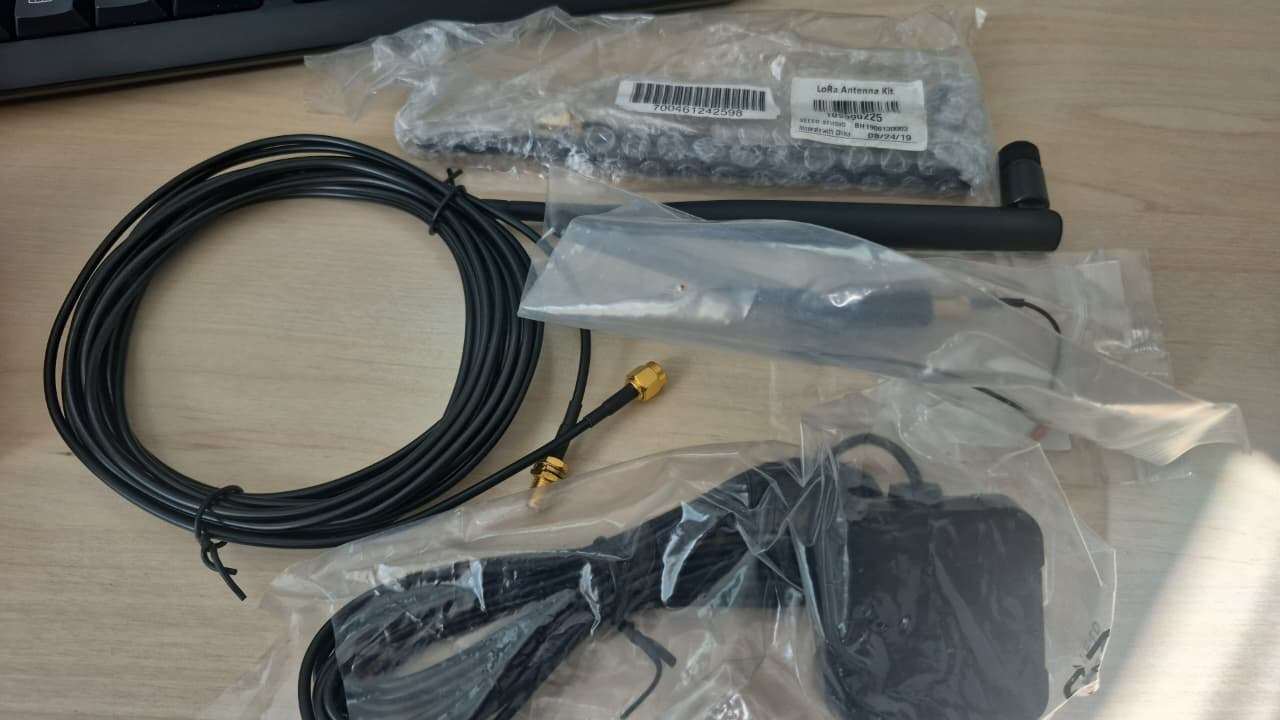
\includegraphics[width=0.94\linewidth]{figuras/kit_antenas_fotografia.jpg}};
  \begin{scope}[x={(img.south east)},y={(img.north west)}]
    \foreach \l/\x/\y in {A/0.57/0.86,B/0.83/0.62,C/0.53/0.44,D/0.87/0.49,E/0.76/0.24} {
      \node[circle,fill=MAPrimaryDark,text=white,font=\sffamily\bfseries\small,inner sep=1.6pt,draw=white,line width=0.8pt] at (\x,\y) {\l};
    }
  \end{scope}
\end{tikzpicture}
\caption{Accesorios disponibles, fotografiados en el banco (octubre de 2026). Las letras remiten a la tabla~\ref{tab:inventario}. La fotografía documenta el inventario; \emph{no} permite deducir bandas de operación.}
\label{fig:kit}
\end{figure}

{\footnotesize
\begin{longtable}{@{}>{\raggedright\arraybackslash}p{0.13\linewidth}>{\raggedright\arraybackslash}p{0.18\linewidth}>{\raggedright\arraybackslash}p{0.16\linewidth}>{\raggedright\arraybackslash}p{0.15\linewidth}>{\raggedright\arraybackslash}p{0.19\linewidth}>{\raggedright\arraybackslash}p{0.09\linewidth}@{}}
\caption{Inventario fotográfico. «Evidencia visible» es lo que muestra la foto; el resto es identificación con su confianza.}\label{tab:inventario}\\
\toprule
\textbf{Componente} & \textbf{Evidencia visible} & \textbf{Modelo identificado} & \textbf{Frecuencia} & \textbf{Compatibilidad de conexión} & \textbf{Confianza} \\
\midrule
\endfirsthead
\toprule
\textbf{Componente} & \textbf{Evidencia visible} & \textbf{Modelo identificado} & \textbf{Frecuencia} & \textbf{Compatibilidad de conexión} & \textbf{Confianza} \\
\midrule
\endhead
A. Bolsa del kit & Etiqueta «LoRa Antenna Kit», código «109990225», texto «SEEED STUDIO», lote «BH1906130003», fecha 09/24/19 & Seeed Studio 109990225 «LoRa Antenna Kit» & No impresa. Un distribuidor no la especifica & Un distribuidor declara terminación \textbf{RP-SMA macho}: verificar & Media (código legible) \\
B. Antena tipo «rubber duck» & Antena negra con articulación en ángulo & Antena del kit A (probable) & Desconocida; LoRa suele usar 868 o 915 MHz, \emph{no confirmado} & Depende del centro del conector: pin = SMA, agujero = RP-SMA (figura~\ref{fig:conectores}) & Media \\
C. Cable coaxial largo & Cable negro delgado, varias vueltas; un extremo con tuerca dorada, otro con conector roscado de panel & Extensión coaxial, tipo de cable no visible & Desconocida; pérdidas no documentadas & Macho a hembra; SMA o RP-SMA sin confirmar & Media \\
D. Cable en bolsa & Cable delgado con terminal pequeño & Posible \emph{pigtail} U.FL/IPEX a SMA/RP-SMA & Desconocida & U.FL no conecta al HackRF; no usar & Baja \\
E. Antena cuadrada con cable & Carcasa plana negra y cable largo enrollado & No identificada (podría ser una antena activa GNSS o una antena LoRa de panel) & Desconocida & Conector no visible. Si fuese activa, necesitaría alimentación DC & Baja \\
\bottomrule
\end{longtable}
}

\begin{importante}[No deduzca la banda por la forma]
La etiqueta «LoRa» \textbf{no} establece compatibilidad con FM (88--108 MHz) ni con ADS-B (1090 MHz). Aunque la antena B fuese de 868/915 MHz, su comportamiento a 1090 MHz (un 19--26~\% por encima) y a 100 MHz (unas nueve veces por debajo) no está documentado. Este manual la trata como \emph{no calificada} y diseña los procedimientos para que el resultado sea honesto con cualquier rendimiento.
\end{importante}

\subsection{Conectores: la comprobación que más tiempo ahorra}

\begin{figure}[H]
\centering
\resizebox{\linewidth}{!}{% Identificación de conectores: vista frontal esquemática (no a escala).
% Pin = círculo relleno; receptáculo = anillo hueco.
\begin{tikzpicture}[
  cuerpo/.style={draw=MAInk,line width=0.8pt,fill=white},
  rosca/.style={draw=MAMuted,line width=0.5pt,dash pattern=on 1.2pt off 1pt},
  pin/.style={fill=MAInk},
  hueco/.style={draw=MAInk,line width=0.9pt,fill=white},
  tit/.style={font=\sffamily\scriptsize\bfseries,color=MAInk,align=center},
  sub/.style={font=\sffamily\scriptsize,color=MAMuted,align=center}]
  \def\conector#1#2#3#4#5{% #1 x, #2 nombre, #3 detalle, #4 tipo centro (pin|hueco), #5 rosca (ext|int)
    \begin{scope}[shift={(#1,0)}]
      \ifthenelse{\equal{#5}{ext}}{\draw[cuerpo] (0,0) circle (6.5mm); \draw[rosca] (0,0) circle (5.6mm);}
                                  {\draw[cuerpo] (0,0) circle (6.5mm); \draw[rosca] (0,0) circle (7.3mm);}
      \draw[draw=MAMuted,fill=MASurfaceAlt] (0,0) circle (3.3mm);
      \ifthenelse{\equal{#4}{pin}}{\fill[pin] (0,0) circle (0.75mm);}{\draw[hueco] (0,0) circle (0.9mm);}
      \node[tit] at (0,-11mm) {#2};
      \node[sub] at (0,-16.5mm) {#3};
    \end{scope}}
  \conector{0}{SMA hembra}{HackRF ANTENNA\\pin: receptáculo}{hueco}{ext}
  \conector{3.15}{SMA macho}{tuerca + \textbf{pin}\\compatible con el HackRF}{pin}{int}
  \conector{6.3}{RP-SMA macho}{tuerca + \textbf{receptáculo}\\\textcolor{MADanger}{sin contacto central}}{hueco}{int}
  \conector{9.45}{RP-SMA hembra}{rosca exterior + pin\\(típico de Wi-Fi/LoRa)}{pin}{ext}
  \begin{scope}[shift={(12.75,0)}]
    \draw[cuerpo] (0,0) circle (8mm); \draw[rosca] (0,0) circle (7mm);
    \draw[draw=MAMuted,fill=MASurfaceAlt] (0,0) circle (4.2mm);
    \draw[hueco] (0,0) circle (1.1mm);
    \node[tit] at (0,-11mm) {N hembra};
    \node[sub] at (0,-16.5mm) {SIGLENT RF INPUT\\requiere adaptador};
  \end{scope}
  \node[sub,anchor=west,align=left] at (-0.8,-23mm) {Rosca exterior: anillo punteado interior al cuerpo. Tuerca (rosca interior): anillo punteado exterior.\\
    Regla práctica: mire el centro del conector del accesorio. \textbf{Pin} macizo $\Rightarrow$ SMA macho (sirve). \textbf{Agujero} $\Rightarrow$ RP-SMA macho (no sirve sin adaptador).};
\end{tikzpicture}
}
\caption{Identificación de conectores en vista frontal (esquema, no a escala). Un RP-SMA macho enroscado en el SMA hembra del HackRF \emph{no} establece contacto central: la antena queda prácticamente desconectada, sin daño, pero la recepción será casi nula y engañosa.}
\label{fig:conectores}
\end{figure}

El analizador tiene entrada \textbf{tipo N hembra} (hoja de datos SSA3000X Plus). Ningún accesorio del kit tiene conector N. Para llevar una antena SMA al analizador hace falta un adaptador \textbf{N macho -- SMA hembra} (para antena SMA macho) o \textbf{N macho -- RP-SMA hembra} (para antena RP-SMA macho). SIGLENT lo incluye en el accesorio opcional \emph{Utility Kit} (UKitSSA3X), pero su presencia en el banco \textbf{no está confirmada}. Las actividades con el analizador dependen de ese adaptador (tabla~\ref{tab:decision}).

\subsection{Longitud eléctrica y pérdidas del cable}

La longitud de onda es $\lambda = c/f$. Una antena resonante simple mide del orden de $\lambda/4$ (monopolo) o $\lambda/2$ (dipolo):

\begin{longtable}{@{}lrrr@{}}
\toprule
\textbf{Frecuencia} & $\boldsymbol{\lambda}$ & $\boldsymbol{\lambda/4}$ & \textbf{Uso} \\
\midrule
\endhead
100 MHz & 3,00 m & 75 cm & FM comercial (Lab.\ 01) \\
868 MHz & 34,5 cm & 8,6 cm & LoRa (Europa) \\
915 MHz & 32,8 cm & 8,2 cm & LoRa (América) \\
1090 MHz & 27,5 cm & 6,9 cm & ADS-B/Mode S (Lab.\ 02) \\
\bottomrule
\end{longtable}

Una antena de unos 17--20 cm es eléctricamente muy corta a 100 MHz. Aun así, las emisoras de FM locales suelen ser intensas, así que la recepción \emph{puede} funcionar: hay que comprobarlo. A 1090 MHz la desadaptación es menor, pero las señales de aeronaves lejanas son débiles y las paredes y ventanas las atenúan.

El cable C añade pérdidas. Como orden de magnitud, un coaxial delgado tipo RG-174 pierde del orden de 0,2~dB/m a 100 MHz y del orden de 0,6--0,7~dB/m a 1 GHz (valores típicos de fabricantes; el tipo exacto del cable C no está documentado). Unos 3~m a 1090 MHz cuestan unos 2~dB: casi siempre compensa si permiten llevar la antena a una ventana con vista despejada.

\subsection{Decisión de preparación del hardware}
\label{sec:decision}

\begin{longtable}{@{}>{\raggedright\arraybackslash}p{0.25\linewidth}>{\raggedright\arraybackslash}p{0.18\linewidth}>{\raggedright\arraybackslash}p{0.49\linewidth}@{}}
\caption{Decisión por configuración. \PASS: documentada y adecuada. \COND: puede funcionar, sin calificar. \BLOQ: incompatible o insegura hasta resolver lo indicado.}\label{tab:decision}\\
\toprule
\textbf{Configuración} & \textbf{Decisión} & \textbf{Motivo y condición para avanzar} \\
\midrule
\endfirsthead
\toprule
\textbf{Configuración} & \textbf{Decisión} & \textbf{Motivo y condición para avanzar} \\
\midrule
\endhead
Antena B con conector \textbf{SMA macho} (pin) $\rightarrow$ HackRF, FM 88--108 MHz & \COND & Antena eléctricamente corta y sin especificación en FM. Se valida en clase: audio inteligible de al menos una emisora local. \\
Antena B con conector \textbf{RP-SMA macho} (agujero) $\rightarrow$ HackRF & \BLOQ & Sin contacto central. Requiere adaptador RP-SMA hembra -- SMA macho, \emph{no} disponible. Use el respaldo de cada laboratorio. \\
Antena B $\rightarrow$ HackRF, 1090 MHz & \COND & Fuera de la banda nominal probable. Solo una prueba con tramas válidas (nivel 4) la califica \emph{para ese lugar}. \\
Antena B $\rightarrow$ adaptador N $\rightarrow$ SIGLENT & \COND\ / \BLOQ & \COND\ si el adaptador existe; \BLOQ\ si no. Sin adaptador, las mediciones con el analizador se sustituyen por la demostración del instructor o se aplazan. \\
Antena E (no identificada) & \BLOQ & Identificar modelo y conector antes de usarla. \textbf{Nunca} active el \gui{Bias tee} para «probar» una antena desconocida. \\
Pigtail D (U.FL) & \BLOQ & El U.FL no conecta ni al HackRF ni al analizador; es frágil (pocos ciclos de conexión). \\
Cualquier unión HackRF $\leftrightarrow$ SIGLENT & \BLOQ & Fuera del alcance de este manual de solo recepción. \\
\bottomrule
\end{longtable}

\begin{nota}[Recomendación de compra, condicional]
Para una recepción en vivo \emph{predecible} se recomienda adquirir (no existen hoy en el banco): (1) adaptadores N macho -- SMA hembra y RP-SMA hembra -- SMA macho; (2) para el Laboratorio 02, una antena especificada para 1090 MHz (monopolo $\lambda/4$ con plano de tierra o colineal), conector SMA macho, ROE $\le 2{:}1$ en 1085--1095 MHz e impedancia de 50~$\Omega$; (3) un cable de bajas pérdidas si la antena irá a más de 2--3~m. Un monopolo de $\lambda/4$ hecho con coaxial y radiales de $\approx$ 6,9~cm es un proyecto clásico de bajo coste, pero no está calificado en este manual.
\end{nota}

\section{Puerta de seguridad RF}
\label{sec:seguridad}

\begin{alerta}[Solo recepción]
Ningún paso de este manual transmite. Están \textbf{prohibidos}: cualquier transmisión FM radiada o conducida; transmitir ADS-B, Mode S o interrogaciones SSR (1030/1090 MHz); cualquier emisión de prueba en bandas aeronáuticas; agregar en SDRangel dispositivos \gui{HackRF Output} o canales moduladores; y conectar una salida RF activa (incluida la salida TG del analizador) a una entrada sensible. Interferir en 1030/1090 MHz afecta a sistemas de seguridad de vuelo.
\end{alerta}

\begin{longtable}{@{}>{\raggedright\arraybackslash}p{0.27\linewidth}>{\raggedright\arraybackslash}p{0.33\linewidth}>{\raggedright\arraybackslash}p{0.32\linewidth}@{}}
\caption{Límites de entrada y fuente de cada dato.}\label{tab:limites}\\
\toprule
\textbf{Equipo / puerto} & \textbf{Límite documentado} & \textbf{Consecuencia práctica} \\
\midrule
\endfirsthead
\caption[]{(continuación)}\\
\toprule
\textbf{Equipo / puerto} & \textbf{Límite documentado} & \textbf{Consecuencia práctica} \\
\midrule
\endhead
HackRF One, puerto ANTENNA (RX) & Máximo $-5$~dBm; superarlo puede causar daño permanente (documentación oficial HackRF One) & Nunca conectar a una salida de generador, transmisor o TG. Mantener \gui{RF Amp} apagado salvo indicación \\
HackRF One, alimentación de antena & 3,0--3,3~V, máximo 50~mA, controlada por software (documentación HackRF) & \gui{Bias tee} desactivado siempre: puede dañar antenas con cortocircuito en DC o equipos conectados \\
SIGLENT SSA3032X Plus, RF INPUT & Tipo N hembra, 50~$\Omega$. Potencia media máx.\ 30~dBm (3 min, $f_c \ge 10$~MHz, ATT $> 20$~dB, preamp.\ apagado); daño a 33~dBm; DC máx.\ $\pm 50$~V (hoja de datos DS0703P) & Con antena pasiva los niveles reales son órdenes de magnitud menores; el riesgo práctico es la descarga electrostática y la sobrecarga con el preamplificador activado \\
SIGLENT, salida TG (opcional) & Hasta 0~dBm en el SSA3032X Plus si la opción está instalada & Mantener el TG \textbf{apagado} y su puerto libre \\
\bottomrule
\end{longtable}

\begin{alerta}[Orden de conexión y buenas prácticas]
\begin{enumerate}
  \item Toque una superficie metálica conectada a tierra antes de manipular conectores (descarga electrostática). No toque el pin central.
  \item Conecte y desconecte la antena con el receptor \textbf{detenido} en SDRangel o con el analizador encendido pero sin barrido de medida crítica. Apriete los SMA a mano, sin herramientas: girar el cuerpo del cable en lugar de la tuerca daña el pin.
  \item Inspeccione los cables antes de usarlos: sin cortes, dobleces bruscos ni pines torcidos. Un conector dañado se retira.
  \item No acerque transmisores (radios portátiles, nodos LoRa, teléfonos en llamada) a menos de unos metros de la antena del HackRF.
  \item \textbf{Emplazamientos aeroportuarios:} el HackRF no tiene preselección; las interrogaciones de un radar secundario (1030 MHz) llegan a su entrada aunque esté sintonizado en otra frecuencia. Estimación de orden de magnitud: con una potencia de pico radiada típica de unos 90 dBm y una pérdida de espacio libre de unos 93 dB a 1 km, el pico recibido por una antena de 0 dBi ronda $-4$ dBm, comparable al límite de $-5$ dBm. A menos de unos pocos kilómetros de un SSR o un DME: \gui{RF amp} siempre apagado y consulte al instructor antes de instalar la antena en exterior.
  \item Si el HackRF o el analizador se calientan de forma anómala o huelen a quemado, desconecte la alimentación y avise al instructor.
\end{enumerate}
\end{alerta}

\section{Preparación previa y requisitos}
\label{sec:prerrequisitos}

\begin{longtable}{@{}>{\raggedright\arraybackslash}p{0.22\linewidth}>{\raggedright\arraybackslash}p{0.72\linewidth}@{}}
\toprule
\textbf{Quién} & \textbf{Qué debe estar listo antes de la sesión} \\
\midrule
\endhead
Instructor & Software instalado y probado en cada puesto; decisión de hardware de la tabla~\ref{tab:decision} completada; grabación de respaldo verificada; adaptador N confirmado o actividad del analizador replanificada. Detalle en la \emph{Guía del instructor}. \\
Estudiante & Conceptos: frecuencia y longitud de onda, decibelios (dB, dBm), ancho de banda, muestreo, AM/FM, radar primario y secundario. Los laboratorios de Python del repositorio (Laboratorio 02, secciones 1, 3, 4, 7 y 8) los cubren. Habilidades: abrir una terminal, copiar órdenes con exactitud, guardar capturas de pantalla. \\
Estudiante, recomendado & Leer este capítulo completo y responder el cuestionario diagnóstico del laboratorio antes de llegar. \\
\bottomrule
\end{longtable}

\section{Estado de validación de esta edición}
\label{sec:estado}

\begin{estado}
\begin{itemize}
  \item \textbf{Verificado con documentación oficial:} versiones (SDRangel 7.27.2 del 19-08-2026; HackRF host 2026.01.3; paquete \texttt{hackrf} 2023.01.1 de Ubuntu 24.04), límites de entrada del HackRF y del analizador, nombres de plugins y controles de SDRangel, formato \texttt{.sdriq}.
  \item \textbf{Ejecutado en software (Windows 11, 15-10-2026):} SDRangel 7.27.2 para Windows leyó la grabación de respaldo del Laboratorio 02 con \gui{FileInput} y el \gui{ADS-B Demodulator} decodificó la aeronave ICAO 4D2023 «AMC421» con posiciones correctas. Dos decodificadores independientes confirmaron las tramas.
  \item \textbf{No ejecutado:} instalación en Ubuntu 24.04, cualquier operación con el HackRF One real, recepción FM en vivo, recepción ADS-B en vivo y mediciones con el SIGLENT. La interfaz gráfica de SDRangel se describió con su documentación y su API, no con capturas.
  \item \textbf{Consecuencia:} la calidad documental fue revisada; la validación en campo con el hardware del banco está \textbf{pendiente} y la hace el instructor antes de clase.
\end{itemize}
\end{estado}
